\section{Justificación}

Se configura una paradoja pedagógica. El currículo oficial (Lineamientos, Estándares y DBA) establece con claridad que la trigonometría debe vincularse con pensamiento variacional, modelación e interpretación de fenómenos \parencite{ministeriodeeducacionnacionalLineamientosCurriculares1998,ministeriodeeducacionnacionalEstandaresBasicos2006,ministeriodeeducacionnacionalDerechosBasicos2016}. En ese marco, no basta con calcular correctamente: se espera interpretación, argumentación y articulación entre formas de representación. Ese proceso debería iniciarse desde el álgebra en noveno y consolidarse en décimo y undécimo.

En consecuencia, resulta pertinente preguntar por qué las evaluaciones nacionales e internacionales siguen mostrando las mismas brechas \parencite{ministeriodeeducacionnacionalmenInformeNacionalSaber2019, icfesProgramaParaEvaluacion2024}. Los datos de PISA entre 2006 y 2022 ilustran el problema con precisión. En el plano de los puntajes promedio (Figura~\ref{fig:pisa_promedio}), Colombia pasó de 370 a 383 puntos en matemáticas a lo largo de dieciséis años: un avance de 13 puntos mientras el promedio de la OCDE se mantenía sistemáticamente cerca de los 490 puntos. En 2022, la brecha entre Colombia y el promedio de la OCDE era de 89 puntos, más de ocho veces la ganancia acumulada por el país en toda la serie histórica.

\begin{figure}[H]
  \centering
  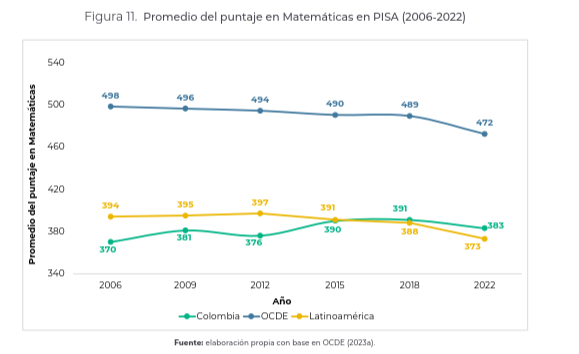
\includegraphics[width=0.88\textwidth]{imagenes/00Figuras/pisa_promedio_puntaje_2006_2022.png}
  \caption{Promedio del puntaje en Matemáticas en PISA (2006--2022) para Colombia, Latinoamérica y la OCDE.
  Tomado de \textcite{icfesProgramaParaEvaluacion2024}.}
  \label{fig:pisa_promedio}
\end{figure}

Más revelador aún es el análisis por niveles de desempeño (Figura~\ref{fig:pisa_niveles}). En 2006, el 72\,\% de los estudiantes colombianos se ubicaba por debajo del nivel~2 —el umbral que la OCDE considera competencia matemática básica—. En 2022, esa cifra era del 71\,\%: dieciséis años de reformas curriculares, nuevos estándares y diversas iniciativas pedagógicas produjeron un desplazamiento de apenas un punto porcentual. En el extremo opuesto, menos del 1\,\% de los estudiantes colombianos alcanza los niveles 5 o~6 —los que corresponden a razonamiento matemático avanzado—, frente al 31\,\% que lo logra en los países de la OCDE. La distribución de desempeño de Colombia en 2022 es prácticamente idéntica a la de 2006.

\begin{figure}[H]
  \centering
  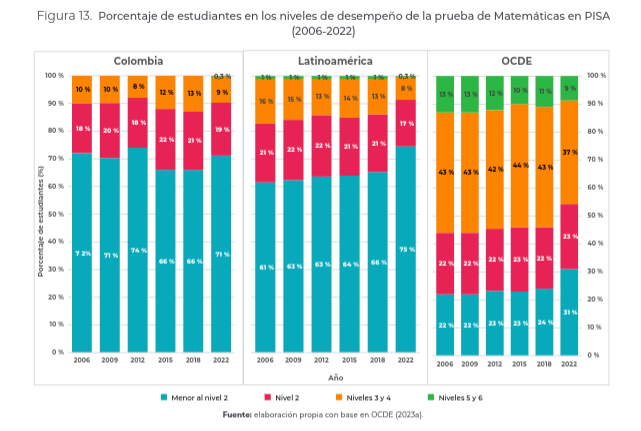
\includegraphics[width=0.88\textwidth]{imagenes/00Figuras/pisa_niveles_desempeno_2006_2022.png}
  \caption{Porcentaje de estudiantes en los niveles de desempeño de la prueba de Matemáticas en PISA (2006--2022). Colombia permanece con más del 70\,\% de estudiantes por debajo del nivel~2 a lo largo de toda la serie.
  Tomado de \textcite{icfesProgramaParaEvaluacion2024}.}
  \label{fig:pisa_niveles}
\end{figure}

Estos datos no implican que el currículo sea erróneo. Implican que el currículo ha prescrito un tipo de razonamiento matemático que las prácticas pedagógicas predominantes no han logrado producir. Una respuesta consistente en la literatura señala la distancia entre lo que el currículo prescribe y lo que efectivamente se desarrolla en el aula.

Los estudios didácticos han documentado que, cuando predominan ejercicios cerrados ---con solución directa y predecible---, se reduce el espacio para la duda, la conjetura y la argumentación. En tales condiciones, el avance en pensamiento matemático profundo es limitado \parencite{fiallolealAcercaInvestigacionEducacion2015,delgadoEstrategiaDidacticaPara2023,zubietaTipificacionErroresDificultades2018}. Modificar esta situación exige rediseñar las tareas para que demanden exploración, comparación de decisiones y análisis del error como parte del aprendizaje.

En este contexto, la IA no se plantea como solución automática, sino como apoyo al diseño didáctico. Puede ofrecer retroalimentación oportuna y abrir rutas diferenciadas según las necesidades del estudiante. Sin embargo, su potencial depende de que la tarea conserve exigencia matemática. Cuando la IA solo automatiza prácticas repetitivas, el aporte pedagógico es mínimo \parencite{romeroalonsoRolInteligenciaArtificial2024,castillodelpezoUseArtificialIntelligence2024,parrasanchezPersonalizacionRecursosPara2023}.

Desde esta perspectiva, el estudio se orienta a comprender qué ocurre cuando se diseñan e implementan tareas de trigonometría con exigencia matemática y apoyo de IA en un contexto escolar real. El interés se centra en identificar qué decisiones didácticas funcionan, dónde aparecen bloqueos y cómo la IA puede aportar sin desplazar el protagonismo del razonamiento matemático del estudiante.
